% =============================================================
%  Đề án Chiến lược Công ty
%  Strategic Plan — AI Agent Systems for Knowledge-Intensive Workflows
%  Đà Nẵng, 2026 — Internal strategy document
%  Biên dịch: xelatex chien-luoc-cong-ty.tex
% =============================================================
\documentclass[11pt,a4paper]{article}

\usepackage[margin=2.2cm,top=2cm,bottom=2.2cm]{geometry}
\usepackage{fontspec}
\usepackage{tikz}
\usepackage{xcolor}
\usepackage{tabularx}
\usepackage{booktabs}
\usepackage{enumitem}
\usepackage{titlesec}
\usepackage{fancyhdr}
\usepackage{hyperref}
\usepackage{setspace}
\usepackage{tcolorbox}
\tcbuselibrary{skins, breakable}
\usetikzlibrary{positioning, shapes.geometric, shapes.misc, arrows.meta,
                fit, calc, decorations.pathreplacing, backgrounds, chains, scopes}

\setmainfont{Latin Modern Roman}
\setsansfont{Latin Modern Sans}

% ---------- colors ----------
\definecolor{ink}{HTML}{14213d}
\definecolor{accent}{HTML}{fca311}
\definecolor{mid}{HTML}{8d99ae}
\definecolor{ok}{HTML}{2a9d8f}
\definecolor{warn}{HTML}{c44536}
\definecolor{soft}{HTML}{f4f1de}
\definecolor{leaf}{HTML}{3d5a80}
\definecolor{cool}{HTML}{5e6472}

\hypersetup{colorlinks=true, linkcolor=ink, urlcolor=leaf}

\titleformat{\section}{\sffamily\bfseries\LARGE\color{ink}}{Chương \thesection.}{0.5em}{}
\titleformat{\subsection}{\sffamily\bfseries\large\color{ink}}{\thesubsection}{0.5em}{}
\titleformat{\subsubsection}{\sffamily\bfseries\normalsize\color{ink}}{}{0em}{}
\titlespacing*{\section}{0pt}{1.4em}{0.6em}
\titlespacing*{\subsection}{0pt}{1.0em}{0.3em}
\titlespacing*{\subsubsection}{0pt}{0.6em}{0.2em}

\setlist{nosep, leftmargin=1.3em, topsep=3pt, itemsep=2pt}
\setlength{\parskip}{4pt}
\setlength{\parindent}{0pt}
\onehalfspacing

\pagestyle{fancy}
\fancyhf{}
\fancyhead[L]{\sffamily\footnotesize\color{mid} Đề án Chiến lược Công ty}
\fancyhead[R]{\sffamily\footnotesize\color{mid} Internal \textbullet{} 2026}
\fancyfoot[C]{\sffamily\footnotesize\color{mid}\thepage}
\renewcommand{\headrulewidth}{0pt}

\newtcolorbox{keybox}[1][]{
  enhanced, colback=soft, colframe=accent, boxrule=0.5pt,
  left=8pt, right=8pt, top=5pt, bottom=5pt, arc=1pt,
  fonttitle=\sffamily\bfseries\color{ink}, #1
}
\newtcolorbox{warnbox}[1][]{
  enhanced, colback=warn!8, colframe=warn, boxrule=0.5pt,
  left=8pt, right=8pt, top=5pt, bottom=5pt, arc=1pt,
  fonttitle=\sffamily\bfseries\color{warn}, #1
}
\newtcolorbox{framebox_}[1][]{
  enhanced, colback=leaf!6, colframe=leaf, boxrule=0.5pt,
  left=8pt, right=8pt, top=5pt, bottom=5pt, arc=1pt,
  fonttitle=\sffamily\bfseries\color{leaf}, #1
}
\newtcolorbox{quotebox}[1][]{
  enhanced, colback=white, colframe=ink!30, boxrule=0pt,
  borderline west={2pt}{0pt}{ink},
  left=10pt, right=8pt, top=4pt, bottom=4pt, arc=0pt, #1
}

\begin{document}

% =============================================================
% TITLE PAGE
% =============================================================
\thispagestyle{empty}
\vspace*{3cm}
\begin{center}
{\sffamily\bfseries\fontsize{30}{36}\selectfont\color{ink} Đề án Chiến lược}\\[0.3em]
{\sffamily\bfseries\fontsize{30}{36}\selectfont\color{ink} Công ty}\\[1em]
{\sffamily\Large\color{mid} AI Agent Systems for Knowledge-Intensive Workflows}\\[0.3em]
{\sffamily\large\color{mid} Việt Nam \textbullet{} Đông Nam Á \textbullet{} 2026--2030}\\[4em]

\begin{tikzpicture}[font=\sffamily\footnotesize]
  \node[rectangle, draw=ink, thick, rounded corners=2pt, fill=soft, minimum width=3cm, minimum height=1.2cm, align=center] (a) at (0,0) {\textbf{Khát vọng}\\\scriptsize Aspiration};
  \node[rectangle, draw=ink, thick, rounded corners=2pt, fill=soft, minimum width=3cm, minimum height=1.2cm, align=center] (b) at (3.5,0) {\textbf{Nơi chơi}\\\scriptsize Where to Play};
  \node[rectangle, draw=ink, thick, rounded corners=2pt, fill=soft, minimum width=3cm, minimum height=1.2cm, align=center] (c) at (7,0) {\textbf{Cách thắng}\\\scriptsize How to Win};
  \node[rectangle, draw=ink, thick, rounded corners=2pt, fill=soft, minimum width=3cm, minimum height=1.2cm, align=center] (d) at (10.5,0) {\textbf{Năng lực}\\\scriptsize Capabilities};
  \node[rectangle, draw=ink, thick, rounded corners=2pt, fill=soft, minimum width=3cm, minimum height=1.2cm, align=center] (e) at (14,0) {\textbf{Quản trị}\\\scriptsize Management};
  \draw[-{Latex[length=2.5mm]}, thick, ink] (a) -- (b);
  \draw[-{Latex[length=2.5mm]}, thick, ink] (b) -- (c);
  \draw[-{Latex[length=2.5mm]}, thick, ink] (c) -- (d);
  \draw[-{Latex[length=2.5mm]}, thick, ink] (d) -- (e);
\end{tikzpicture}

\vspace{1em}
{\small\itshape\color{mid} Chuỗi quyết định chiến lược (Playing to Win — Lafley \& Martin)}

\vspace{3em}
{\sffamily\color{mid} Đà Nẵng, tháng 4 năm 2026}
\end{center}
\vfill
\begin{center}
{\footnotesize\itshape\color{mid}
Tài liệu này là bản chiến lược chính thức của công ty — dùng để định hướng\\
quyết định đầu tư, sản phẩm, bán hàng, và vận hành trong 3 năm tới.}
\end{center}
\clearpage

\tableofcontents
\clearpage

% =============================================================
% TÓM TẮT CHIẾN LƯỢC — ONE PAGE
% =============================================================
\section*{Tóm tắt chiến lược}
\addcontentsline{toc}{section}{Tóm tắt chiến lược}

\begin{keybox}[title=Chiến lược một câu]
Chúng tôi xây \textbf{hệ thống AI Agent tự vận hành có kiểm soát} cho các tổ chức
tri thức tại Việt Nam, thắng bằng cách \textbf{hiểu sâu workflow vertical} hơn các
công ty công nghệ phổ quát, và \textbf{nhanh hơn} các công ty outsourcing truyền thống
nhờ framework nội bộ tái sử dụng.
\end{keybox}

\textbf{5 quyết định chiến lược cốt lõi (Playing to Win)}

\begin{enumerate}
\item \textbf{Khát vọng.} Trong 5 năm, là công ty hàng đầu Đông Nam Á về \textit{Agent
Systems cho ngành dịch vụ tri thức}, đo bằng: 50--100 khách doanh nghiệp \& tổ
chức giáo dục, doanh thu 30--50 tỷ VND/năm, biên lợi nhuận gộp 50\%+.

\item \textbf{Nơi chơi.} Đại học tư thục và bán công Việt Nam tầm trung
(3.000--15.000 sinh viên) $\to$ dịch vụ du lịch/y tế tư nhân $\to$ Đông Nam Á.
\textit{Không đụng:} public sector, K-12, fintech, tập đoàn Fortune 500.

\item \textbf{Cách thắng.} Vertical depth (hiểu nghiệp vụ sâu hơn) $+$ Framework
leverage (triển khai nhanh hơn agency) $+$ Vietnamese context (ngôn ngữ, văn hoá,
quy trình) $+$ Network effects (benchmark dữ liệu xuyên khách hàng).

\item \textbf{Năng lực cốt lõi cần xây.} (a) Agent engineering chất lượng
production, (b) Discovery \& workflow design cho giáo dục VN, (c) Evals \&
governance đạt chuẩn doanh nghiệp, (d) Land-and-expand GTM motion, (e) Partner
ecosystem với trường đại học.

\item \textbf{Hệ thống quản trị.} Cơ chế 3-chữ-ký; decision gates M6/M12/M24/M36;
quarterly strategy review; rolling 12-month plan.
\end{enumerate}

\textbf{Lộ trình 3 giai đoạn}

\begin{tabularx}{\linewidth}{@{}p{2.8cm} X@{}}
\toprule
\textbf{Giai đoạn 1 (M1--M12) — Prove} & 1 vertical (giáo dục). 2 use case (Admissions + Internal Knowledge). 2--3 design partner trả phí. Framework v1.0. Doanh thu 500M--1B VND. \\
\textbf{Giai đoạn 2 (M13--M24) — Scale} & Solution packaging. 10--15 khách. Thời gian delivery 6--8 tuần/khách. Thử vertical 2. Doanh thu 3--5B VND. \\
\textbf{Giai đoạn 3 (M25--M36) — Platform} & Subscription v1. 30--50 khách. Mở rộng ĐNA. Biên lợi nhuận 40--50\%. Doanh thu 15--25B VND. \\
\bottomrule
\end{tabularx}

\clearpage

% =============================================================
% PART I — BỨC TRANH CHIẾN LƯỢC
% =============================================================
\begin{center}
\vspace*{0.5em}
{\sffamily\bfseries\Huge\color{ink} Phần I}\\[0.5em]
{\sffamily\LARGE\color{mid} Bức tranh chiến lược}\\[0.5em]
{\color{mid}\rule{6cm}{0.4pt}}
\end{center}
\vspace{1em}

% =============================================================
\section{Khát vọng \& Định nghĩa thành công}

\subsection{Khát vọng (Winning Aspiration)}

\begin{quotebox}
\textit{Trong 5 năm, chúng tôi muốn trở thành công ty \textbf{đầu tiên được nhớ
đến} ở Đông Nam Á khi một tổ chức tri thức --- trường đại học, doanh nghiệp dịch
vụ, hãng du lịch --- quyết định ``agentify'' workflow của họ.}
\end{quotebox}

Khát vọng này có 3 tầng:

\begin{itemize}
\item \textbf{Tầng sản phẩm.} Là công ty được đánh giá cao nhất về \textit{độ tin
cậy vận hành} (uptime, accuracy, governance), không phải về \textit{độ mới của
công nghệ}.
\item \textbf{Tầng thương hiệu.} Là ``Stripe của agent systems cho ngành dịch
vụ tri thức tại ĐNA'' --- tức là chọn được vì chất lượng infrastructure, không
phải vì giá rẻ hay tính năng nhiều.
\item \textbf{Tầng tổ chức.} Là công ty 30--50 người, lợi nhuận dương, không phụ
thuộc một round gọi vốn nào --- tức là tồn tại được bằng kinh tế thật.
\end{itemize}

\subsection{Định nghĩa thành công — 3 năm và 5 năm}

\begin{tabularx}{\linewidth}{@{}p{3.5cm} X X@{}}
\toprule
\textbf{Chỉ số} & \textbf{Thành công 3 năm} & \textbf{Thành công 5 năm} \\
\midrule
Khách hàng & 30--50 tổ chức, 80\%+ giáo dục & 50--100 tổ chức, đa vertical \\
Doanh thu & 15--25 tỷ VND/năm & 30--50 tỷ VND/năm \\
Doanh thu lặp lại (ARR) & 40\% tổng doanh thu & 70\%+ tổng doanh thu \\
Biên lợi nhuận gộp & 40--50\% & 55--65\% \\
Net dollar retention & 110\%+ & 120\%+ \\
Nhân sự & 20--30 người & 30--50 người \\
Vị trí địa lý & Việt Nam + 1--2 khách ĐNA & 4--5 quốc gia ĐNA \\
Thương hiệu & Top-3 VN về agent systems & Top-3 ĐNA \\
Framework reuse rate & 70\%+ qua các dự án & 85\%+ \\
\bottomrule
\end{tabularx}

\subsection{Đặt cược chiến lược (The Strategic Bet)}

Một công ty không thể thắng ở mọi mặt trận. Sau khi phân tích thị trường và khả
năng, đây là đặt cược chính của chúng tôi:

\begin{framebox_}[title=The Bet]
\textit{Trong 3--5 năm tới, các tổ chức tri thức cỡ vừa tại Việt Nam và Đông Nam
Á sẽ chi đáng kể để \textbf{tự động hoá workflow tri thức}. Cửa sổ này đủ dài để
một công ty xuất phát từ Đà Nẵng với \textbf{hiểu biết vertical sâu} và \textbf{
framework được tái sử dụng} có thể chiếm được 5--10\% thị phần phân khúc này trước
khi các big tech toàn cầu hoặc các công ty công nghệ lớn Việt Nam quyết định
nghiêm túc về phân khúc này.}
\end{framebox_}

Nếu đặt cược này đúng: công ty có cơ hội trở thành vertical leader.\\
Nếu đặt cược này sai: công ty vẫn có thể sống được như một boutique AI
consultancy 10--15 người.

\textbf{Downside protection} của chúng tôi là kinh tế vận hành tốt ngay từ năm 2
--- không phụ thuộc vào gọi vốn lớn để tồn tại.

\clearpage

% =============================================================
\section{Phân tích thị trường \& Cơ hội}

\subsection{Thị trường tổng thể (TAM / SAM / SOM)}

\begin{tabularx}{\linewidth}{@{}p{2.8cm} X p{3cm}@{}}
\toprule
\textbf{Lớp thị trường} & \textbf{Phạm vi} & \textbf{Quy mô ước tính} \\
\midrule
\textbf{TAM} --- Tổng & Enterprise AI agents toàn cầu & \$100--200B/năm (2030) \\
\textbf{SAM-1} --- Khu vực & Enterprise AI agents Đông Nam Á & \$2--4B/năm (2030) \\
\textbf{SAM-2} --- Ngành & Agent systems cho dịch vụ tri thức ĐNA & \$500M--1B/năm \\
\textbf{SOM} --- Thực tế & Giáo dục \& dịch vụ tri thức VN tầm trung & \$50--100M/năm \\
\bottomrule
\end{tabularx}

\textbf{Vì sao SOM là con số thật đáng quan tâm (không phải TAM):}
\begin{itemize}
\item Chúng tôi không cần TAM để thành công. Chúng tôi cần chiếm 5--10\% SOM ở Việt Nam.
\item 5--10\% SOM = 2.5--10M USD/năm doanh thu tại Việt Nam, đủ cho công ty 30--50 người.
\item TAM chỉ là tín hiệu rằng thị trường đủ lớn để không ``chạm trần'' trong 10 năm tới.
\end{itemize}

\subsection{Phân tích 5 lực lượng của Porter (cho phân khúc giáo dục VN)}

\begin{tabularx}{\linewidth}{@{}p{4cm} p{1.8cm} X@{}}
\toprule
\textbf{Lực lượng} & \textbf{Mức độ} & \textbf{Ý nghĩa chiến lược} \\
\midrule
Đối thủ hiện hữu & \textbf{Thấp} & Thị trường chưa có công ty chuyên agent systems cho giáo dục VN. Công ty outsourcing lớn bận với tập đoàn lớn. \\
Người mới vào & \textbf{Trung bình} & Big tech (OpenAI, Anthropic, Google) chưa ưu tiên VN giáo dục. Startup mới cần 18--24 tháng để đuổi kịp về vertical depth. \\
Quyền lực khách hàng & Trung bình & Trường đại học có budget nhưng quy trình mua chậm. Cần pilot → proof → scale. \\
Quyền lực nhà cung cấp & \textbf{Cao} & Phụ thuộc vào foundation model (OpenAI, Anthropic). \textbf{Rủi ro cao nhất.} \\
Sản phẩm thay thế & Trung bình & Hiện tại: manual process, chatbot đơn giản, hoặc ``in-house tự làm''. Không có sản phẩm thay thế ngang hàng. \\
\bottomrule
\end{tabularx}

\textbf{Kết luận Porter:} Cấu trúc ngành hiện tại \textbf{rất thuận lợi cho người
vào sớm có vertical depth}. Rủi ro lớn nhất là phụ thuộc nhà cung cấp model, cần
có chiến lược giảm thiểu (xem Chương 9).

\subsection{Phân tích timing --- Vì sao là bây giờ}

\begin{center}
\begin{tikzpicture}[font=\sffamily, scale=1]
  % Timeline
  \draw[ink!50, very thick] (0,0) -- (14,0);
  \foreach \x/\y in {0/2022, 3/2024, 6/2026, 9/2028, 12/2030} {
    \draw[ink!50, thick] (\x,0.15) -- (\x,-0.15);
    \node[below=1mm, font=\footnotesize] at (\x,-0.15) {\y};
  }

  % Phases
  \draw[decorate, decoration={brace, amplitude=5pt}, cool, thick] (0,0.5) -- (2.5,0.5)
    node[midway, above=5pt, font=\footnotesize\sffamily] {Chatbot};
  \draw[decorate, decoration={brace, amplitude=5pt}, cool, thick] (2.7,0.5) -- (5.5,0.5)
    node[midway, above=5pt, font=\footnotesize\sffamily] {Copilot};
  \draw[decorate, decoration={brace, amplitude=5pt}, ok, thick, ultra thick] (5.7,0.5) -- (9,0.5)
    node[midway, above=5pt, font=\footnotesize\sffamily\bfseries, ok] {CỬA SỔ AGENT};
  \draw[decorate, decoration={brace, amplitude=5pt}, cool, thick] (9.2,0.5) -- (12,0.5)
    node[midway, above=5pt, font=\footnotesize\sffamily] {Saturation};

  % Our window
  \fill[ok, opacity=0.15] (5.7,-0.8) rectangle (9,-0.3);
  \node[font=\footnotesize\sffamily\bfseries, ok] at (7.3,-0.55) {Cửa sổ để xác lập vị thế};

  % Events
  \node[font=\tiny\sffamily, ink!70] at (0,-1.2) {GPT-3.5};
  \node[font=\tiny\sffamily, ink!70] at (3,-1.2) {GPT-4 / Claude};
  \node[font=\tiny\sffamily, ink!70, text width=2.5cm, align=center] at (6,-1.2) {Agent SDKs chín\\Tool-use ổn};
  \node[font=\tiny\sffamily, ink!70, text width=2.5cm, align=center] at (9,-1.2) {Big tech vào\\vertical};
\end{tikzpicture}
\end{center}

\textbf{Cửa sổ thời gian} để công ty vertical-specific xác lập vị thế là
2026--2028, khoảng 2--3 năm. Sau đó, cạnh tranh sẽ chuyển từ ``có vào được
không'' sang ``phòng thủ vị thế đã có''. Đây là lý do chúng tôi ưu tiên
\textbf{tốc độ chiếm design partner} hơn là \textbf{tối ưu hoá sản phẩm}.

\subsection{Insight về khách hàng giáo dục Việt Nam}

Sau discovery sơ bộ, chúng tôi thấy 5 insight quan trọng:

\begin{enumerate}
\item \textbf{Pain lớn nhất không phải ``thiếu công nghệ''} --- mà là \textbf{
quá tải người vận hành}. Phòng tuyển sinh, phòng công tác sinh viên, phòng đào
tạo đều bị ngập câu hỏi lặp lại.

\item \textbf{Khách hàng sợ ``AI ảo'' và ``AI đọc linh tinh''} --- không sợ
công nghệ. Họ cần \textit{trust}, không cần \textit{wow}. Citations, audit
trail, và human-in-the-loop quan trọng hơn độ thông minh.

\item \textbf{Ra quyết định: 3 tầng.} (a) Trưởng phòng đề xuất; (b) Phó hiệu
trưởng / CFO duyệt; (c) Hiệu trưởng ký. Chu kỳ 2--4 tháng. Cần tài liệu cho cả 3 tầng.

\item \textbf{Ngân sách CNTT tại trường tư tầm trung:} 500M--3B VND/năm. 10--20\%
có thể dành cho AI / tự động hoá nếu có ROI rõ ràng.

\item \textbf{Thời điểm mua tốt nhất}: sau học kỳ (tháng 1--2, 6--7) khi có
data và có ngân sách năm mới. \textbf{Tồi nhất}: giữa mùa tuyển sinh (tháng
3--5, 8--9).
\end{enumerate}

\clearpage

% =============================================================
\section{Định vị: Nơi chơi (Where to Play)}

\subsection{Bản đồ định vị thị trường}

\begin{center}
\begin{tikzpicture}[font=\sffamily, scale=1]
  % Axes
  \draw[-{Latex[length=2.5mm]}, thick, ink] (0,0) -- (12,0) node[right, font=\footnotesize\sffamily] {Hiểu ngành};
  \draw[-{Latex[length=2.5mm]}, thick, ink] (0,0) -- (0,7.5) node[above, font=\footnotesize\sffamily] {Độ sâu kỹ thuật agent};
  \node[font=\tiny\sffamily, ink!70] at (1.5,-0.4) {thấp};
  \node[font=\tiny\sffamily, ink!70] at (10.5,-0.4) {cao};
  \node[font=\tiny\sffamily, ink!70, rotate=90] at (-0.4,1.5) {thấp};
  \node[font=\tiny\sffamily, ink!70, rotate=90] at (-0.4,6) {cao};

  % Competitors
  \node[circle, draw=ink, fill=mid!40, minimum size=11mm, align=center, font=\tiny\sffamily] at (8,2) {Big\\tech};
  \node[circle, draw=ink, fill=mid!40, minimum size=11mm, align=center, font=\tiny\sffamily] at (2,2) {Chatbot\\VN};
  \node[circle, draw=ink, fill=mid!40, minimum size=11mm, align=center, font=\tiny\sffamily] at (3,5) {AI startup\\horizontal};
  \node[circle, draw=ink, fill=mid!40, minimum size=11mm, align=center, font=\tiny\sffamily] at (9,4) {Agency /\\outsourcing};
  \node[circle, draw=ink, fill=mid!40, minimum size=11mm, align=center, font=\tiny\sffamily] at (5,3) {EduTech\\VN};

  % Us
  \node[circle, draw=ok, very thick, fill=ok!40, minimum size=16mm, align=center, font=\footnotesize\sffamily\bfseries, ink] at (9.5,6) {Chúng\\ta};
  \node[below=2mm of {(9.5,6)}, font=\scriptsize\sffamily, ok] at (9.5,5.1) {vertical depth + framework};

  % Arrows showing defensibility
  \draw[dashed, ok, thick] (9.5,6) circle (1.8);
\end{tikzpicture}
\end{center}

Vị trí chúng tôi chọn là \textbf{góc ``hiểu ngành sâu + độ sâu kỹ thuật cao''}
--- đây là góc không ai đang phục vụ. Các đối thủ hiện tại:

\begin{itemize}
\item \textbf{Big tech (OpenAI, Anthropic, Google):} Kỹ thuật mạnh, hiểu ngành kém, không ưu tiên VN.
\item \textbf{Chatbot VN (FPT.AI, Vbee, cốt lõi NLP Việt):} Không phải agent systems thật sự, kỹ thuật hạn chế.
\item \textbf{AI startup horizontal (ở HN/HCM):} Tập trung tool tổng quát, không vertical depth.
\item \textbf{Agency / outsourcing:} Làm theo yêu cầu, không có framework tái sử dụng, giá cao/delivery chậm.
\item \textbf{EduTech VN (VioEdu, Ehoc):} Tập trung học tập, không phải quản trị/vận hành nhà trường.
\end{itemize}

\subsection{Chọn khách hàng (Customer Choice)}

\subsubsection*{ICP (Ideal Customer Profile) --- năm 1}

\begin{itemize}
\item \textbf{Loại tổ chức:} Đại học tư thục hoặc bán công tại Việt Nam.
\item \textbf{Quy mô:} 3.000--15.000 sinh viên.
\item \textbf{Địa lý:} Tier-1 (Hà Nội, TP.HCM, Đà Nẵng) và Tier-2 (Huế, Cần Thơ, Hải Phòng, Quy Nhơn).
\item \textbf{Ngân sách CNTT:} $\geq$ 500 triệu VND/năm cho AI / tự động hoá.
\item \textbf{Tín hiệu sẵn sàng:} Đã có website tuyển sinh, CRM / SIS, đã thử chatbot đơn giản nhưng chưa hài lòng.
\item \textbf{Người ra quyết định tiếp cận được:} Phó hiệu trưởng chuyên môn, trưởng phòng tuyển sinh, hoặc giám đốc CNTT.
\end{itemize}

\subsubsection*{Mở rộng ICP --- năm 2--3}

\begin{itemize}
\item \textbf{Năm 2:} Mở rộng sang trường công tầm trung có phòng hợp tác doanh nghiệp chủ động. Bắt đầu thử 1--2 khách du lịch / dịch vụ.
\item \textbf{Năm 3:} Du lịch tư nhân (resort, hãng tour), y tế tư nhân cao cấp (phòng khám, thẩm mỹ). Mở rộng ra Đông Nam Á (trường quốc tế và đại học tư thục Philippines, Indonesia, Thailand).
\end{itemize}

\subsection{Chọn sản phẩm (Product Scope Choice)}

\subsubsection*{Làm cái gì (What we do)}

\begin{itemize}
\item Discovery, workflow design, và implementation của agent systems.
\item Custom integration với hệ thống sẵn có của khách (CRM, SIS, LMS, Drive).
\item Operation, monitoring, và continuous improvement (managed services).
\item Training và enablement cho đội ngũ khách hàng.
\end{itemize}

\subsubsection*{Không làm (What we explicitly DO NOT do)}

\begin{itemize}
\item \textbf{Không làm general-purpose AI copilot} --- cạnh tranh trực tiếp với Microsoft, Google, Notion.
\item \textbf{Không làm AI tutoring / student-facing} --- UX và go-to-market hoàn toàn khác.
\item \textbf{Không làm foundation model} --- sử dụng Claude / OpenAI / Gemini.
\item \textbf{Không làm consumer AI} --- B2B only.
\item \textbf{Không làm pure API / dev tools} --- Chúng tôi bán outcome, không bán API.
\item \textbf{Không làm tích hợp low-code / no-code platform} (Zapier, Make-style) --- khác phân khúc.
\end{itemize}

\subsection{Chọn địa lý (Geography Choice)}

\begin{tabularx}{\linewidth}{@{}p{2cm} X p{3.5cm}@{}}
\toprule
\textbf{Thời điểm} & \textbf{Địa lý} & \textbf{Lý do} \\
\midrule
Năm 1 & Việt Nam, ưu tiên Đà Nẵng + miền Trung & Network sẵn có, chi phí vận hành thấp, ít cạnh tranh local. \\
Năm 2 & Toàn Việt Nam + 1 khách pilot ĐNA & Đã có case study, đủ sức bán ra Hà Nội / TP.HCM. \\
Năm 3 & 3--4 nước ĐNA (PH, ID, TH + 1 khác) & Thị trường ngôn ngữ gần, cùng kiểu doanh nghiệp SMB-mid. \\
Năm 5 & Đông Nam Á rộng hơn + thử Nhật/Hàn & Sau khi có quy mô ĐNA đủ lớn. \\
\bottomrule
\end{tabularx}

\textbf{Không làm:} Mỹ, châu Âu, Trung Quốc trong 5 năm đầu. Lý do: cạnh tranh
quá đậm, chi phí sales quá cao, không có lợi thế so sánh.

\clearpage

% =============================================================
\section{Cách thắng (How to Win)}

\subsection{Câu chuyện thắng (The Winning Formula)}

\begin{keybox}[title=Công thức thắng]
\textbf{Vertical depth} (hiểu workflow giáo dục VN sâu)\\
$+$ \textbf{Framework leverage} (triển khai nhanh, chi phí thấp)\\
$+$ \textbf{Vietnamese context by default} (ngôn ngữ, văn hoá, quy định)\\
$+$ \textbf{Network effects} (benchmark xuyên khách hàng)\\
$=$ Công ty dẫn đầu phân khúc vertical trong 3 năm.
\end{keybox}

\subsection{4 nguồn lợi thế cạnh tranh}

\subsubsection*{Lợi thế 1 --- Vertical depth}

Không công ty công nghệ phổ quát nào hiểu được:
\begin{itemize}
\item Quy chế tuyển sinh chi tiết của Bộ GD\&ĐT và cách từng trường diễn giải khác nhau.
\item Các khái niệm CĐR, PLO, CLO, rubric --- cách một trường thật sự đánh giá chất lượng.
\item Văn hoá ``hỏi đi hỏi lại'' của phụ huynh / sinh viên VN, khác hẳn khách hàng phương Tây.
\item Chu kỳ tuyển sinh 3 tháng cao điểm + 9 tháng low-season.
\end{itemize}

Đây là kiến thức \textbf{cần 2--3 năm lặn ngụp trong ngành} để có được. Big tech
không bỏ công; horizontal AI startup không đủ động lực.

\subsubsection*{Lợi thế 2 --- Framework leverage}

\begin{itemize}
\item Framework 6 khối (Knowledge / Workflow / Tools / Reasoning / Evals / Governance) được xây từ dự án đầu tiên.
\item Từ dự án thứ 3, tái sử dụng $\geq$ 60\% code/config.
\item Từ dự án thứ 6, tái sử dụng $\geq$ 80\%.
\item \textbf{Hệ quả kinh tế:} Chi phí biên mỗi khách mới giảm từ 100\% $\to$ 20\%, biên lợi nhuận tăng từ 20\% $\to$ 60\%+.
\item Agency truyền thống \textbf{không có} lợi thế này --- mỗi dự án ≈ mỗi lần làm từ đầu.
\end{itemize}

\subsubsection*{Lợi thế 3 --- Vietnamese context by default}

Khi khách hàng giáo dục VN gặp các sản phẩm toàn cầu, họ luôn phải làm thêm
10--30\% tuỳ chỉnh (dịch, viết lại prompt, tích hợp CRM Việt, xử lý văn bản có
dấu). Chúng tôi loại bỏ khoản này \textbf{mặc định}. Điều này tạo ra 2 lợi ích:

\begin{itemize}
\item Khách hàng onboard nhanh hơn.
\item Trải nghiệm ``đúng ngôn ngữ'' từ đầu, không phải mảng thêm.
\end{itemize}

\subsubsection*{Lợi thế 4 --- Network effects (mở ra từ năm 2)}

Khi có 5+ khách, chúng tôi có thể:
\begin{itemize}
\item Benchmark \textit{anonymously}: ``Trường bạn có tỷ lệ escalation 23\% --- trung bình ngành là 15--18\%''.
\item Chia sẻ \textit{best practice} giữa khách hàng tương đồng.
\item Huấn luyện model nội bộ (small LLM, embeddings) trên dữ liệu tổng hợp (sau khi có contractual quyền).
\end{itemize}

Khách hàng \textbf{mới} muốn vào để \textbf{tận dụng benchmark} --- đây là network effect thật.

\subsection{Cách đối thủ không thể sao chép nhanh}

Ngay cả khi một công ty lớn (FPT, VNG, CMC) muốn vào:
\begin{itemize}
\item \textbf{Họ cần 12--18 tháng} để xây framework tương đương (nhưng sẽ bị sa vào ôm nhiều vertical cùng lúc, pha loãng depth).
\item \textbf{Họ cần 6--12 tháng} để làm 5 design partner đầu --- trong khoảng đó chúng tôi đã có 15--20.
\item \textbf{Họ có incentive ngược}: phải giải trình ROI ngắn hạn với cổ đông lớn, khó kiên trì với phân khúc trung.
\end{itemize}

\subsection{Jobs-to-be-Done: Khách hàng thật sự ``thuê'' chúng tôi để làm gì?}

\begin{tabularx}{\linewidth}{@{}p{4cm} X@{}}
\toprule
\textbf{Functional job} & Giảm 60--80\% câu hỏi routine gửi đến phòng tuyển sinh / công tác sinh viên. \\
\textbf{Emotional job} & Phó hiệu trưởng / trưởng phòng tuyển sinh \textit{không còn cảm thấy bất lực} trước volume câu hỏi mùa cao điểm. \\
\textbf{Social job} & Trường hiện đại, sinh viên và phụ huynh \textit{được đối đãi chuyên nghiệp} --- là một điểm bán cạnh tranh trong tuyển sinh. \\
\bottomrule
\end{tabularx}

Khách hàng \textbf{không thuê} chúng tôi vì ``AI''. Họ thuê chúng tôi vì muốn
giải quyết 3 job trên. Mọi giao tiếp sales, marketing, product phải quay về 3
job này.

\clearpage

% =============================================================
% PART II — CÁC TRỤ CỘT CHIẾN LƯỢC
% =============================================================
\begin{center}
\vspace*{0.5em}
{\sffamily\bfseries\Huge\color{ink} Phần II}\\[0.5em]
{\sffamily\LARGE\color{mid} Các trụ cột chiến lược}\\[0.5em]
{\color{mid}\rule{6cm}{0.4pt}}
\end{center}
\vspace{1em}

% =============================================================
\section{Chiến lược sản phẩm}

\subsection{Kiến trúc sản phẩm 2 lớp}

\begin{center}
\begin{tikzpicture}[
  font=\sffamily,
  sol/.style={draw=ink, fill=accent!25, rounded corners=2pt,
              minimum width=36mm, minimum height=11mm, align=center, inner sep=2pt,
              font=\footnotesize\sffamily},
  solfut/.style={draw=ink!70, fill=accent!5, dashed, rounded corners=2pt,
              minimum width=36mm, minimum height=11mm, align=center, inner sep=2pt,
              font=\footnotesize\sffamily\itshape},
  fwk/.style={draw=ink, fill=mid!30, rounded corners=2pt,
              minimum width=26mm, minimum height=14mm, align=center, inner sep=2pt,
              font=\footnotesize\sffamily},
  infra/.style={draw=ink!60, fill=cool!20, rounded corners=2pt,
              minimum width=30mm, minimum height=9mm, align=center, inner sep=2pt,
              font=\footnotesize\sffamily},
  arr/.style={-{Latex[length=3mm]}, thick, ink!75}
]
  % Layer A
  \node[sol] (a1) at (0,0) {Admissions\\Agent};
  \node[sol, right=3mm of a1] (a2) {Student Services\\Agent};
  \node[sol, right=3mm of a2] (a3) {Internal Knowledge\\Agent};
  \node[solfut, right=3mm of a3] (a4) {Service / Travel\\Agent (Y2+)};

  \node[font=\footnotesize\sffamily\itshape, ink, above=1mm of a1.north west, anchor=south west]
    {LỚP A --- Solutions bán ra (theo vertical, có tên thương hiệu)};

  % Layer B
  \node[fwk, below=16mm of a1.south west, anchor=north west, text width=24mm] (b1)
    {\textbf{Knowledge}\\\scriptsize Ingest, metadata, citation};
  \node[fwk, right=2mm of b1, text width=24mm] (b2)
    {\textbf{Workflow}\\\scriptsize Intake, routing, approval};
  \node[fwk, right=2mm of b2, text width=24mm] (b3)
    {\textbf{Tools}\\\scriptsize Connectors to external systems};
  \node[fwk, right=2mm of b3, text width=24mm] (b4)
    {\textbf{Reasoning}\\\scriptsize Agent orchestration};
  \node[fwk, below=2mm of b2, text width=24mm] (b5)
    {\textbf{Evals}\\\scriptsize Test set, logs, confidence};
  \node[fwk, right=2mm of b5, text width=24mm] (b6)
    {\textbf{Governance}\\\scriptsize Access, audit, policy};

  \node[font=\footnotesize\sffamily\itshape, ink, above=1mm of b1.north west, anchor=south west]
    {LỚP B --- Core Framework (tài sản nội bộ, không bán trực tiếp)};

  % Layer C — infra
  \node[infra, below=16mm of b1.south west, anchor=north west] (c1) {Foundation models\\\scriptsize Claude / GPT / Gemini};
  \node[infra, right=3mm of c1] (c2) {Cloud infrastructure\\\scriptsize AWS / GCP};
  \node[infra, right=3mm of c2] (c3) {Vector DB\\\scriptsize pgvector / Qdrant};
  \node[infra, right=3mm of c3] (c4) {Observability\\\scriptsize Logs / traces / evals};

  \node[font=\footnotesize\sffamily\itshape, ink, above=1mm of c1.north west, anchor=south west]
    {LỚP C --- Infrastructure (mua / dùng, không xây lại)};

  % Arrows
  \draw[arr] ($(b2.east)!0.5!(b3.west)$) ++(0,14mm) -- ++(0,4mm)
      node[right, font=\scriptsize\sffamily\itshape, ink!80]{\;đóng gói};
  \draw[arr] ($(c2.east)!0.5!(c3.west)$) ++(0,7mm) -- ++(0,5mm)
      node[right, font=\scriptsize\sffamily\itshape, ink!80]{\;dùng};
\end{tikzpicture}
\end{center}

\textbf{Nguyên tắc cốt lõi:}

\begin{itemize}
\item \textbf{Lớp A} là cái khách hàng mua --- đặt tên, định giá, có ROI đo được.
\item \textbf{Lớp B} là tài sản nội bộ --- không bán, không đặt tên thương hiệu trong 12--18 tháng đầu. Đây là IP của công ty.
\item \textbf{Lớp C} là infrastructure --- \textbf{không xây lại}. Dùng foundation model tốt nhất, cloud provider ổn, vector DB có sẵn. Chúng tôi không phải Anthropic; không cần xây model riêng.
\end{itemize}

\subsection{Product Roadmap 3 năm}

\begin{tabularx}{\linewidth}{@{}p{2cm} X@{}}
\toprule
\textbf{Năm} & \textbf{Sản phẩm lớp A (được bán ra)} \\
\midrule
\textbf{Năm 1} & Admissions Agent v1, Internal Knowledge Agent v1 \\
\textbf{Năm 2} & + Student Services Agent, Academic Ops Agent. Phiên bản v2 của 2 sản phẩm năm 1. \\
\textbf{Năm 3} & + Service Operations Agent (du lịch, dịch vụ). Platform SaaS cho Admissions Agent. \\
\bottomrule
\end{tabularx}

\subsection{Build vs Buy}

\begin{tabularx}{\linewidth}{@{}p{4cm} c X@{}}
\toprule
\textbf{Năng lực} & \textbf{Quyết định} & \textbf{Lý do} \\
\midrule
Foundation model & \textcolor{warn}{\textbf{BUY}} & Không có lợi thế gì khi tự build. \\
Orchestration / agent framework & \textbf{BUILD} (wrapper) & Lớp B chính là IP. Không dùng nguyên LangChain / CrewAI. \\
Vector DB & \textcolor{warn}{\textbf{BUY}} & pgvector / Qdrant đủ tốt. \\
Vietnamese embeddings fine-tune & \textbf{BUILD} (năm 2) & Là lợi thế Vietnamese context. \\
Observability / evals & \textbf{BUILD (wrapper)} + BUY (base) & Core cho trust. \\
CRM / CMS / LMS & \textcolor{warn}{\textbf{BUY}} (tích hợp) & Khách đã có. \\
Admin dashboard & \textbf{BUILD} & Là giao diện khách thấy hằng ngày. \\
Auth / billing & \textcolor{warn}{\textbf{BUY}} & Clerk / Paddle / Stripe. \\
\bottomrule
\end{tabularx}

\subsection{Technical principles}

\begin{enumerate}
\item \textbf{Model-agnostic where possible.} Lớp B phải hoạt động với 2--3 foundation model khác nhau. Giảm phụ thuộc.
\item \textbf{Evals as first-class.} Không có feature nào được release nếu chưa có test set.
\item \textbf{Human-in-the-loop by default.} Mọi agent có escalation path ngay từ v1.
\item \textbf{Observable by default.} Mọi agent run có log đầy đủ, có thể trace.
\item \textbf{Small before big.} Single agent + good tool > multi-agent khi chưa cần.
\item \textbf{Backwards compatibility.} Một khi khách onboarded, schema không đổi trong tối thiểu 12 tháng.
\end{enumerate}

\clearpage

% =============================================================
\section{Chiến lược Go-to-Market}

\subsection{Motion: Land and Expand}

\begin{center}
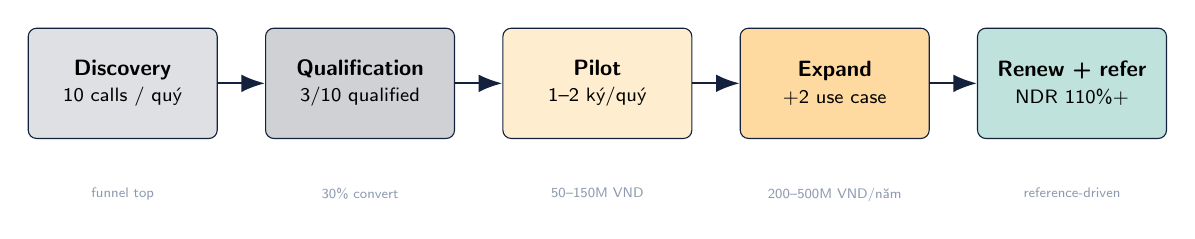
\begin{tikzpicture}[
  font=\sffamily,
  stage/.style={draw=ink, rounded corners=3pt, minimum width=24mm, minimum height=14mm, align=center, inner sep=2pt, font=\footnotesize\sffamily},
  arr/.style={-{Latex[length=3mm]}, thick, ink}
]
  \node[stage, fill=cool!20] (s1) at (0,0) {\textbf{Discovery}\\\scriptsize 10 calls / quý};
  \node[stage, fill=cool!30, right=6mm of s1] (s2) {\textbf{Qualification}\\\scriptsize 3/10 qualified};
  \node[stage, fill=accent!20, right=6mm of s2] (s3) {\textbf{Pilot}\\\scriptsize 1--2 ký/quý};
  \node[stage, fill=accent!40, right=6mm of s3] (s4) {\textbf{Expand}\\\scriptsize +2 use case};
  \node[stage, fill=ok!30, right=6mm of s4] (s5) {\textbf{Renew + refer}\\\scriptsize NDR 110\%+};

  \draw[arr] (s1) -- (s2);
  \draw[arr] (s2) -- (s3);
  \draw[arr] (s3) -- (s4);
  \draw[arr] (s4) -- (s5);

  % Numbers below
  \node[below=5mm of s1, font=\tiny\sffamily] {\textcolor{mid}{funnel top}};
  \node[below=5mm of s2, font=\tiny\sffamily] {\textcolor{mid}{30\% convert}};
  \node[below=5mm of s3, font=\tiny\sffamily] {\textcolor{mid}{50--150M VND}};
  \node[below=5mm of s4, font=\tiny\sffamily] {\textcolor{mid}{200--500M VND/năm}};
  \node[below=5mm of s5, font=\tiny\sffamily] {\textcolor{mid}{reference-driven}};
\end{tikzpicture}
\end{center}

\subsection{Sales motion theo giai đoạn}

\subsubsection*{Giai đoạn 1 (M1--M12): Founder-led sales}

\begin{itemize}
\item \textbf{Ai bán:} Hảo + Hoàng (đi cùng). Hảo mở cửa (warm intro), Hoàng chốt.
\item \textbf{Cách tiếp cận:} Warm introduction > LinkedIn outbound > events.
\item \textbf{Nơi tìm:} Network học thuật của Hảo, alumni, ban giám hiệu, các hội thảo ngành.
\item \textbf{Sales cycle:} 2--4 tháng (từ intro đến ký pilot).
\item \textbf{Chi phí:} Chủ yếu thời gian founder, chưa thuê sales.
\end{itemize}

\subsubsection*{Giai đoạn 2 (M13--M24): Sales-assisted}

\begin{itemize}
\item Tuyển 1 BD đầu tiên cuối Q4 năm 1 / đầu năm 2.
\item Hoàng chuyển vai từ \textit{người bán} sang \textit{head of business} --- train BD, xây playbook, giám sát pipeline.
\item Outbound có hệ thống: 30--50 trường/quý được tiếp cận với tài liệu chuẩn.
\item \textbf{Sales cycle:} Giảm về 1.5--3 tháng nhờ có case study.
\end{itemize}

\subsubsection*{Giai đoạn 3 (M25--M36): Multi-channel}

\begin{itemize}
\item Inbound từ content marketing, thought leadership, events.
\item Reseller / partner channel (công ty tư vấn giáo dục, nhà phân phối CNTT).
\item Direct outbound với BDR + AE chuyên biệt (2--3 người).
\item Khởi động self-serve cho Admissions Agent (tier thấp nhất).
\end{itemize}

\subsection{Positioning \& Messaging}

\subsubsection*{3 tầng message theo người nghe}

\begin{tabularx}{\linewidth}{@{}p{3.5cm} X@{}}
\toprule
\textbf{Người nghe} & \textbf{Message chính} \\
\midrule
Hiệu trưởng / Phó hiệu trưởng & ``Trường bạn hiện đại trong mắt phụ huynh, sinh viên giữ chân tốt hơn, nhân sự hạnh phúc hơn.'' (Outcome thương hiệu \& nhân sự) \\
Trưởng phòng tuyển sinh / CTSV & ``Giảm 60--80\% câu hỏi lặp lại, bạn có thể dành thời gian làm việc chiến lược.'' (Outcome công việc hằng ngày) \\
Giám đốc CNTT & ``Tích hợp sẵn, có audit trail, không làm phức tạp hệ thống hiện tại.'' (Outcome kỹ thuật \& rủi ro) \\
\bottomrule
\end{tabularx}

\subsubsection*{Những điều KHÔNG nói}

\begin{itemize}
\item Không dùng ``framework'', ``multi-agent'', ``LLM'' khi bán.
\item Không hứa ``thay thế con người''.
\item Không dùng buzzword (``cách mạng'', ``đột phá'', ``tương lai'').
\item Không so sánh trực tiếp với ChatGPT / Gemini.
\end{itemize}

\subsection{Marketing \& Thought Leadership}

Năm 1 không đầu tư lớn marketing. Tập trung:

\begin{itemize}
\item \textbf{1 case study/quý} sau khi có design partner đầu.
\item \textbf{2--3 blog post/tháng} trên LinkedIn \& blog công ty (Hảo chủ trì content).
\item \textbf{1 webinar/quý} cho trưởng phòng tuyển sinh / CNTT.
\item \textbf{1 hội thảo lớn/năm} --- ``AI cho quản trị giáo dục'' tại Đà Nẵng, mời 30--50 trường.
\end{itemize}

\clearpage

% =============================================================
\section{Mô hình kinh doanh \& Kinh tế đơn vị}

\subsection{Mô hình doanh thu theo giai đoạn}

\begin{tabularx}{\linewidth}{@{}p{2.8cm} X X@{}}
\toprule
\textbf{Giai đoạn} & \textbf{Cái được bán} & \textbf{Giá} \\
\midrule
\textbf{G1: Design partner} & Discovery workshop + pilot 8--12 tuần + 3 tháng managed operation & 50--150M VND/pilot \\
\textbf{G2: Packaged solution} & Solution chuẩn (Admissions / SS / IK) + custom onboarding + 1 năm operation & 200--500M VND/trường/năm \\
\textbf{G3: Subscription} & SaaS subscription theo tier (Starter / Pro / Enterprise) + add-on & 100--800M VND/trường/năm \\
\bottomrule
\end{tabularx}

\subsection{Kinh tế đơn vị (Unit Economics)}

\subsubsection*{Unit economics --- khách trung bình giai đoạn 2 (ước tính)}

\begin{tabularx}{\linewidth}{@{}p{5.5cm} r X@{}}
\toprule
\textbf{Chỉ số} & \textbf{Giá trị} & \textbf{Ghi chú} \\
\midrule
Giá trị hợp đồng năm 1 (ACV) & 300M VND & Solution + onboarding + ops \\
Giá trị hợp đồng năm 2+ (ACV) & 280M VND & Ops + upsell, không có onboarding \\
Gross margin năm 1 & 30\% & Nhiều tuỳ chỉnh thủ công \\
Gross margin năm 2+ & 60\% & Framework đã tái sử dụng \\
Customer acquisition cost (CAC) & 50--80M VND & Chủ yếu thời gian founder \\
Payback period & 6--10 tháng & Dựa trên gross profit năm 1 \\
Net dollar retention (NDR) & 110\%+ & Upsell use case thứ 2, 3 \\
Lifetime (năm, ước tính) & 4--5 năm & Switching cost cao sau năm 2 \\
LTV (customer lifetime value) & 800M--1.2B VND & Cumulative gross profit \\
LTV : CAC ratio & 10--15$\times$ & Rất khoẻ nếu đạt được \\
\bottomrule
\end{tabularx}

\textbf{Lý do LTV:CAC cao:} founder-led sales giai đoạn đầu có CAC thấp, và
switching cost khi khách đã tích hợp workflow sâu là cao.

\subsection{Dự báo tài chính 3 năm}

\begin{tabularx}{\linewidth}{@{}p{4.5cm} r r r@{}}
\toprule
\textbf{(Tỷ VND)} & \textbf{Năm 1} & \textbf{Năm 2} & \textbf{Năm 3} \\
\midrule
Số khách mới & 2--3 & 8--10 & 15--20 \\
Số khách tích luỹ & 2--3 & 10--13 & 25--30 \\
Doanh thu & 0.5--1.0 & 3--5 & 15--25 \\
Doanh thu lặp lại (ARR) & 0 & 1--2 & 6--10 \\
Chi phí nhân sự & 0.6--0.9 & 2.5--3.5 & 8--12 \\
Chi phí vận hành (cloud, tools) & 0.1--0.2 & 0.3--0.5 & 1--2 \\
EBITDA & -0.5 đến 0 & -0.5 đến +0.5 & +2 đến +5 \\
Nhân sự cuối năm & 3--4 & 10--12 & 22--28 \\
\bottomrule
\end{tabularx}

\subsection{Chiến lược gọi vốn}

\subsubsection*{Nguyên tắc:}

\begin{enumerate}
\item \textbf{Không gọi seed round} nếu không cần thiết trong 12--18 tháng đầu.
Founder equity dưới 70\% sớm sẽ làm suy yếu động lực và quyền tự quyết.

\item \textbf{Gọi vốn khi có bằng chứng, không trước.} Tiêu chí tối thiểu để
gọi pre-A: 8--10 khách, ARR $\geq$ 3 tỷ, NDR $\geq$ 100\%, team $\geq$ 8 người.

\item \textbf{Ưu tiên angel \& strategic} hơn VC institutional trong 24 tháng đầu.
\end{enumerate}

\subsubsection*{Lộ trình gọi vốn đề xuất}

\begin{tabularx}{\linewidth}{@{}p{2.8cm} X X@{}}
\toprule
\textbf{Round} & \textbf{Thời điểm} & \textbf{Mục đích} \\
\midrule
Bootstrap + founder & M1--M12 & Runway 9--12 tháng. Không gọi vốn ngoài. \\
Angel round (tuỳ chọn) & M12--M18 & 2--5 tỷ VND, angel hoặc strategic từ giáo dục. Mục đích: mở rộng sales. \\
Pre-Series A & M24--M30 & 20--40 tỷ VND từ VC khu vực. Mục đích: scale ĐNA. \\
Series A & M36+ & 80--150 tỷ VND, chỉ khi platform play rõ. \\
\bottomrule
\end{tabularx}

\clearpage

% =============================================================
\section{Chiến lược cạnh tranh \& Moat}

\subsection{Phân tích 7 Powers (Hamilton Helmer)}

\begin{tabularx}{\linewidth}{@{}p{3cm} c X@{}}
\toprule
\textbf{Power} & \textbf{Có / Chưa} & \textbf{Đánh giá} \\
\midrule
Scale economies & Sau Y3 & Với 50+ khách, chi phí cố định (framework, evals) phân bổ thấp xuống. \\
Network effects & \textbf{Có, từ Y2} & Benchmark xuyên khách, best-practice sharing, aggregate training. \\
Counter-positioning & \textbf{Có ngay từ Y1} & Big tech không thể ôm phân khúc vertical VN vì economics ngược. \\
Switching costs & \textbf{Có ngay từ sau pilot} & Workflow tích hợp sâu + dữ liệu lịch sử $\Rightarrow$ rời đi cost $>$ 500M. \\
Branding & Sau Y3 & Cần thời gian và case study. \\
Cornered resource & \textbf{Một phần, từ Y1} & Network học thuật của Hảo là warm intro hiếm có. \\
Process power & \textbf{Có, từ Y2} & Framework delivery chuẩn hoá; agency không có. \\
\bottomrule
\end{tabularx}

\textbf{Diễn giải:} Chúng tôi có \textbf{4--5 trên 7 powers} ở năm 2, đặc biệt
mạnh về \textit{counter-positioning, switching costs, process power}. Đây là
tổ hợp đủ để xây vị thế vertical leader.

\subsection{Counter-positioning: tại sao big tech không thể đuổi theo}

\begin{center}
\begin{tikzpicture}[font=\sffamily\footnotesize]
  \node[rectangle, draw=ink, rounded corners=2pt, fill=soft, minimum width=5cm, minimum height=1cm, align=center] (a) at (0,0) {\textbf{Big tech (OpenAI, Google, FPT)}\\\scriptsize doanh thu cao, quy mô lớn};
  \node[rectangle, draw=ink, rounded corners=2pt, fill=ok!20, minimum width=5cm, minimum height=1cm, align=center] (b) at (8,0) {\textbf{Chúng ta}\\\scriptsize doanh thu nhỏ, margin cao};

  \node[rectangle, draw=warn, rounded corners=2pt, fill=warn!10, minimum width=11cm, minimum height=1.5cm, align=center, below=1cm of $(a)!0.5!(b)$] (c) {\textbf{Phân khúc giáo dục tư VN:} 500M--5B/khách/năm\\\scriptsize Quá nhỏ để big tech ưu tiên. Vừa đủ lớn để chúng ta sống khoẻ.};

  \draw[-{Latex[length=2.5mm]}, thick, warn] (a.south) -- ++(0,-0.4) node[right, font=\tiny]{bỏ qua};
  \draw[-{Latex[length=2.5mm]}, thick, ok] (b.south) -- ++(0,-0.4) node[left, font=\tiny]{ưu tiên};
\end{tikzpicture}
\end{center}

Big tech có \textbf{business model incompatibility}: họ cần phân khúc có \$10M+
ACV để lý giải cost sales force. Phân khúc của chúng tôi (300--500M VND = 12--20K
USD/khách) là \textit{dưới ngưỡng} của họ. Ngay cả khi họ muốn, cấu trúc chi
phí sẽ giết chiến lược.

\subsection{Switching costs: Làm sao khách khó rời đi}

Sau 12 tháng dùng, khách có 4 loại switching cost:

\begin{enumerate}
\item \textbf{Data lock-in:} Knowledge base đã được ingest, phân loại, citation. Chuyển sang vendor khác = mất 2--3 tháng re-ingest.
\item \textbf{Workflow integration:} Agent đã tích hợp vào CRM, LMS, email. Tháo dỡ = re-do 4--6 tuần integration.
\item \textbf{Trained evals:} Test set đã được xây riêng cho trường này. Không transfer được.
\item \textbf{Team familiarity:} Nhân viên đã quen với admin dashboard, reporting. Đào tạo lại tốn công.
\end{enumerate}

\textbf{Ước tính:} Switching cost $\geq$ 500M VND sau 12 tháng. Lớn hơn ACV --- khách hàng lý trí sẽ ở lại trừ khi có lý do chính đáng.

\subsection{Phản ứng trước các kịch bản cạnh tranh}

\begin{tabularx}{\linewidth}{@{}p{5cm} X@{}}
\toprule
\textbf{Kịch bản} & \textbf{Phản ứng chiến lược} \\
\midrule
FPT / VNG tung sản phẩm tương tự & Nhắm khách lớn hơn phân khúc của chúng ta. Giữ vertical depth bằng hiểu biết nghiệp vụ. \\
Startup mới (quốc tế) vào VN & Bảo vệ vị thế bằng local network, language, và khách đã lock-in. \\
Big tech launches vertical solution & Co-opetition: trở thành implementation partner của họ nếu hợp lý. \\
Khách hàng yêu cầu giảm giá 30--50\% do cạnh tranh & Không giảm. Bổ sung value (thêm use case) thay vì giảm giá. \\
Foundation model đổi giá/policy đột ngột & Đã có kiến trúc model-agnostic; chuyển sang model khác trong 2--4 tuần. \\
\bottomrule
\end{tabularx}

\clearpage

% =============================================================
\section{Năng lực cốt lõi cần xây}

\subsection{5 năng lực cốt lõi (Core Capabilities)}

\begin{tabularx}{\linewidth}{@{}p{5cm} X X@{}}
\toprule
\textbf{Năng lực} & \textbf{Vì sao cần} & \textbf{Mức độ hiện tại} \\
\midrule
1. Agent engineering production-grade & Là năng lực lõi kỹ thuật & Khởi điểm (cần xây từ Y1) \\
2. Discovery \& workflow design giáo dục VN & Là nguồn vertical depth & Trung bình (Hảo có base) \\
3. Evals, governance, observability & Là nền của trust & Thấp (cần đầu tư sớm) \\
4. Land-and-expand GTM motion & Là engine tăng trưởng & Thấp (Hoàng có nền tảng B2B) \\
5. Partner ecosystem (trường, tổ chức) & Là đòn bẩy reach & Trung bình (network Hảo) \\
\bottomrule
\end{tabularx}

\subsection{Kế hoạch xây năng lực theo năm}

\begin{tabularx}{\linewidth}{@{}p{2cm} X@{}}
\toprule
\textbf{Năm} & \textbf{Đầu tư năng lực chính} \\
\midrule
\textbf{Năm 1} & Agent engineering (100\%), Discovery workflow (80\%), Evals cơ bản (60\%). GTM \& partner ở mức founder-led. \\
\textbf{Năm 2} & Evals \& governance lên production-grade. Tuyển 1 BD, xây sales playbook. Bắt đầu partner formal với 1--2 trường lớn. \\
\textbf{Năm 3} & Process chuẩn hoá toàn công ty. Data science / ML in-house cho network effects. Reseller ecosystem. \\
\bottomrule
\end{tabularx}

\subsection{Hiring strategy}

\begin{tabularx}{\linewidth}{@{}p{2cm} X X@{}}
\toprule
\textbf{Thời điểm} & \textbf{Vị trí} & \textbf{Lý do} \\
\midrule
M6--M9 & Engineer \#2 (full-time hoặc part-time) & Giảm rủi ro burnout của Phú \\
M10--M12 & Customer Success / Ops (part-time) & Phục vụ 2--3 pilot \\
M13--M15 & Business Development (BD) & Mở rộng outbound \\
M16--M18 & Engineer \#3 & Triển khai 5+ khách song song \\
M19--M24 & Designer, QA / evals lead, Content marketer & Chuẩn hoá product experience \\
\bottomrule
\end{tabularx}

\clearpage

% =============================================================
% PART III — TRIỂN KHAI & KẾT HỢP
% =============================================================
\begin{center}
\vspace*{0.5em}
{\sffamily\bfseries\Huge\color{ink} Phần III}\\[0.5em]
{\sffamily\LARGE\color{mid} Triển khai \& Kết hợp}\\[0.5em]
{\color{mid}\rule{6cm}{0.4pt}}
\end{center}
\vspace{1em}

% =============================================================
\section{Lộ trình 3 năm \& Mốc quyết định}

\subsection{Roadmap tổng thể với decision gates}

\begin{center}
\begin{tikzpicture}[font=\sffamily, scale=1]
  % Timeline
  \draw[ink!60, very thick] (0,0) -- (15.5,0);
  \foreach \x/\m in {0/M1, 2.5/M6, 5/M12, 7.5/M18, 10/M24, 12.5/M30, 15/M36} {
    \draw[ink!60, thick] (\x,0.15) -- (\x,-0.15);
    \node[below=1mm, font=\footnotesize] at (\x,-0.15) {\m};
  }

  % Phases
  \node[rectangle, draw=ink, rounded corners=3pt, fill=cool!25, minimum width=48mm, minimum height=11mm, align=center, font=\footnotesize\sffamily] at (2.5,1.2) {\textbf{GĐ 1: PROVE}\\\scriptsize 1 vertical, 2 use case, pilot};
  \node[rectangle, draw=ink, rounded corners=3pt, fill=accent!30, minimum width=48mm, minimum height=11mm, align=center, font=\footnotesize\sffamily] at (7.5,1.2) {\textbf{GĐ 2: SCALE}\\\scriptsize Packaging, 10--15 khách};
  \node[rectangle, draw=ink, rounded corners=3pt, fill=ok!30, minimum width=48mm, minimum height=11mm, align=center, font=\footnotesize\sffamily] at (12.5,1.2) {\textbf{GĐ 3: PLATFORM}\\\scriptsize SaaS, ĐNA, 30--50 khách};

  % Decision gates (diamond markers above timeline)
  \foreach \x/\label in {2.5/G1, 5/G2, 10/G3, 15/G4} {
    \node[diamond, draw=warn, fill=warn!30, minimum size=7mm, font=\tiny\sffamily\bfseries] at (\x,2.8) {\label};
  }

  % Gate descriptions
  \node[below=2mm of {(2.5,-0.5)}, font=\tiny\sffamily, align=center, text width=3cm] at (2.5,-0.8) {1 khách\\trả phí?};
  \node[below=2mm of {(5,-0.5)}, font=\tiny\sffamily, align=center, text width=3cm] at (5,-0.8) {3 khách +\\framework v1.0?};
  \node[below=2mm of {(10,-0.5)}, font=\tiny\sffamily, align=center, text width=3cm] at (10,-0.8) {10+ khách +\\margin 30\%?};
  \node[below=2mm of {(15,-0.5)}, font=\tiny\sffamily, align=center, text width=3cm] at (15,-0.8) {ARR 40\% +\\ĐNA khách đầu?};
\end{tikzpicture}
\end{center}

\subsection{Giai đoạn 1 (M1--M12): Prove --- Chứng minh}

\textbf{Câu hỏi lớn:} Có khách trả phí và chúng tôi có deliver được không?

\textbf{Targets:}
\begin{itemize}
\item 2--3 design partner trả phí (tối thiểu 50M VND mỗi)
\item Framework 6 khối có v1.0
\item Doanh thu 500M--1B VND
\item Burn rate không quá 1.5B VND
\end{itemize}

\textbf{Ưu tiên:} Tốc độ chiếm design partner $>$ hoàn thiện sản phẩm $>$ thương hiệu.

\subsection{Giai đoạn 2 (M13--M24): Scale --- Nhân rộng}

\textbf{Câu hỏi lớn:} Có thể làm được 10--15 khách mà không quá tải?

\textbf{Targets:}
\begin{itemize}
\item 10--15 khách giáo dục trả phí
\item Doanh thu 3--5 tỷ VND
\item Gross margin $\geq$ 30\%
\item Thời gian delivery/khách mới: 6--8 tuần
\item 1 khách thử vertical 2 (du lịch / dịch vụ)
\end{itemize}

\textbf{Ưu tiên:} Packaging $>$ chiếm thêm khách $>$ vertical 2 $>$ gọi vốn.

\subsection{Giai đoạn 3 (M25--M36): Platform --- Nền tảng hoá}

\textbf{Câu hỏi lớn:} Có thể chuyển từ dịch vụ sang SaaS mà không mất khách?

\textbf{Targets:}
\begin{itemize}
\item 30--50 khách
\item Doanh thu 15--25 tỷ VND
\item $\geq$ 40\% ARR
\item Gross margin $\geq$ 50\%
\item 1--3 khách ĐNA
\end{itemize}

\textbf{Ưu tiên:} SaaS self-serve tier $>$ mở rộng ĐNA $>$ platform extensibility.

\subsection{4 Decision Gates --- Điều kiện để tiếp tục}

\begin{tabularx}{\linewidth}{@{}p{1cm} p{2cm} X X@{}}
\toprule
\textbf{Gate} & \textbf{Thời điểm} & \textbf{Điều kiện để pass} & \textbf{Nếu FAIL} \\
\midrule
G1 & M6 & $\geq$ 1 khách trả phí & Giảm quy mô. Gia hạn G1 đến M9. \\
G2 & M12 & $\geq$ 3 khách + framework v1.0 & Không mở vertical 2. Tập trung giai đoạn 1 thêm 6 tháng. \\
G3 & M24 & $\geq$ 10 khách + margin $\geq$ 30\% & Không tuyển thêm. Không thử SaaS. Tập trung profitability. \\
G4 & M36 & ARR $\geq$ 40\% + 1 khách ĐNA & Lùi kế hoạch ĐNA 12 tháng. \\
\bottomrule
\end{tabularx}

\clearpage

% =============================================================
\section{Cách các trụ cột kết hợp --- Integration}

\subsection{Strategic coherence --- Vì sao các mảng hợp lực}

Một chiến lược tốt không phải tổng các lựa chọn tốt ở từng mảng --- mà là
\textbf{sự cộng hưởng giữa các lựa chọn}. Dưới đây là bản đồ cộng hưởng:

\begin{center}
\begin{tikzpicture}[font=\sffamily, scale=1,
  pillar/.style={rectangle, draw=ink, rounded corners=3pt, minimum width=3.3cm, minimum height=1.6cm, align=center, fill=soft, font=\footnotesize\sffamily},
  core/.style={rectangle, draw=accent, very thick, rounded corners=4pt, minimum width=4.5cm, minimum height=1.5cm, align=center, fill=accent!20, font=\footnotesize\sffamily\bfseries},
  arrow/.style={-{Latex[length=2mm]}, thick, ink!70}
]
  \node[core] (c) at (0,0) {NƠI CHƠI:\\Giáo dục VN tầm trung\\CÁCH THẮNG:\\Vertical depth + Framework};

  \node[pillar] (p1) at (-6,2.5) {\textbf{Sản phẩm}\\\scriptsize 2 lớp: solution + framework\\\scriptsize Admissions Agent first};
  \node[pillar] (p2) at (0,3.3) {\textbf{GTM}\\\scriptsize Founder-led $\to$ BD-led\\\scriptsize Land \& expand};
  \node[pillar] (p3) at (6,2.5) {\textbf{Mô hình}\\\scriptsize Services $\to$ Package $\to$ SaaS\\\scriptsize Gross margin 30\% $\to$ 60\%};
  \node[pillar] (p4) at (-6,-2.5) {\textbf{Moat}\\\scriptsize Switching cost + Network + Process};
  \node[pillar] (p5) at (0,-3.3) {\textbf{Năng lực}\\\scriptsize Engineering + Discovery + Evals};
  \node[pillar] (p6) at (6,-2.5) {\textbf{Quản trị}\\\scriptsize 3-chữ-ký + Gates + Rolling plan};

  \foreach \p in {p1,p2,p3,p4,p5,p6} {
    \draw[arrow] (c) -- (\p);
  }
\end{tikzpicture}
\end{center}

\subsection{5 cặp hợp lực quan trọng}

\subsubsection*{1. Sản phẩm ↔ Moat}

Framework 6 khối không chỉ giúp delivery nhanh --- nó tạo ra 2 moat:
\textbf{switching cost} (khách đã tích hợp workflow) và \textbf{process power}
(chúng tôi làm nhanh/chuẩn hơn agency). Không có framework $\Rightarrow$ không có
2 moat này $\Rightarrow$ chiến lược vỡ.

\subsubsection*{2. GTM ↔ Sản phẩm}

Founder-led sales \textbf{chỉ khả thi} khi sản phẩm có 1--2 use case rõ ràng (không
phải ``bất cứ gì bạn muốn''). Ngược lại, sản phẩm chuẩn hoá \textbf{chỉ có thể}
nếu sales biết từ chối yêu cầu ngoài scope. Đây là vòng thuận.

\subsubsection*{3. Mô hình kinh doanh ↔ Cách thắng}

Vertical depth chỉ \textit{chuyển hoá thành lợi nhuận} nếu chuyển được từ project
sang packaged sang subscription. Ngược lại, subscription \textit{chỉ bền} nếu
có vertical depth để giá trị không bị chatbot generic thay thế.

\subsubsection*{4. Năng lực ↔ Hiring}

Năng lực cốt lõi \#3 (Evals, governance) là năng lực hiện tại thấp nhất. Hiring
priority phải ưu tiên người có kỹ năng này trong M18--M24, không chỉ thêm
engineer.

\subsubsection*{5. Quản trị ↔ Tốc độ}

Cơ chế 3-chữ-ký nghe như \textit{làm chậm công ty}. Thực tế: nó ngăn công ty
rơi vào \textit{trap của agency} (nhận mọi dự án), giữ focus, và duy trì
framework reuse rate cao. Tốc độ \textit{dài hạn} nhanh hơn vì tránh rework.

\subsection{Feedback loops --- Vòng tăng cường}

Ba vòng feedback quan trọng mà chúng tôi muốn kích hoạt:

\begin{enumerate}
\item \textbf{Customer $\to$ Framework:} Mỗi khách mới tạo ra feature / connector / eval mới $\to$ framework mạnh lên $\to$ khách tiếp theo triển khai nhanh hơn.

\item \textbf{Case study $\to$ Sales cycle:} Mỗi case study rút sales cycle 20--30\% $\to$ chi phí sales giảm $\to$ margin tăng $\to$ tái đầu tư vào content marketing.

\item \textbf{Benchmark data $\to$ Network effect:} Càng nhiều khách, benchmark càng giá trị $\to$ khách mới muốn vào vì benchmark $\to$ càng nhiều khách. Vòng này \textit{chỉ khởi động khi có 5+ khách}.
\end{enumerate}

\begin{warnbox}[title=Điều kiện để feedback loop hoạt động]
Nếu \textbf{Gate 2 fail} (không đủ 3 khách ở M12), các feedback loop chưa khởi
động được. Đây là lý do tôi đặt G2 là gate quan trọng nhất.
\end{warnbox}

\clearpage

% =============================================================
\section{Quản trị chiến lược}

\subsection{Nhịp review chiến lược}

\begin{tabularx}{\linewidth}{@{}p{3.5cm} p{2cm} X@{}}
\toprule
\textbf{Review} & \textbf{Nhịp} & \textbf{Nội dung} \\
\midrule
Weekly metrics & Hàng tuần & Pipeline, delivery milestones, tiền mặt. \\
Monthly business review & Hàng tháng & KPI tháng, vấn đề lớn, adjust quý. \\
Quarterly strategy review & Hàng quý & Đánh giá gates, review assumption, adjust roadmap. \\
Semi-annual offsite & 6 tháng & Review chiến lược 3 năm, adjust nếu cần. \\
Annual strategic planning & Hàng năm & Rebuild rolling 12--24 month plan. \\
\bottomrule
\end{tabularx}

\subsection{Strategic dashboard --- 10 chỉ số cốt lõi}

\begin{tabularx}{\linewidth}{@{}p{0.5cm} p{4.5cm} X@{}}
\toprule
\textbf{\#} & \textbf{Chỉ số} & \textbf{Tại sao là ``lead indicator''} \\
\midrule
1 & Số discovery call / tháng & Leading indicator của pipeline 3 tháng sau. \\
2 & Pipeline qualified value & Dự báo doanh thu 4--6 tháng sau. \\
3 & Pilot conversion rate & Phản ánh chất lượng GTM \& sản phẩm. \\
4 & Delivery time / khách mới & Đo framework reuse hiệu quả. \\
5 & Gross margin & Sức khoẻ kinh tế đơn vị. \\
6 & NDR (net dollar retention) & Sức khoẻ khách hàng + chất lượng upsell. \\
7 & Framework reuse rate \% & Kiểm tra vertical leverage đang hoạt động. \\
8 & Eval pass rate & Chất lượng sản phẩm trên production. \\
9 & Runway (tháng) & Buffer sống còn. \\
10 & Founder energy 1--10 & Leading indicator của sustainability đội. \\
\bottomrule
\end{tabularx}

\subsection{Rolling 12-month plan --- Kế hoạch liên tục}

\begin{itemize}
\item Công ty duy trì \textbf{1 kế hoạch 12 tháng} và \textbf{1 kế hoạch 36 tháng}, cả hai cùng tồn tại.
\item Kế hoạch 12 tháng \textbf{được cập nhật mỗi quý}, không phải chỉ đầu năm.
\item Kế hoạch 36 tháng \textbf{được cập nhật mỗi semi-annual offsite}.
\item Cả hai kế hoạch đều có phiên bản ``base case'', ``bull case'', ``bear case''.
\item Mỗi quyết định lớn phải trả lời: ``Nó thay đổi kế hoạch như thế nào?''
\end{itemize}

\subsection{Strategic assumption tracker}

Mỗi 6 tháng, review lại 10 assumption chiến lược cốt lõi:

\begin{enumerate}
\item Giáo dục tư VN sẽ chi cho AI $\geq$ 500M/trường/năm. [mức độ tin cậy: ?]
\item Sales cycle trường tư là 2--4 tháng. [?]
\item Framework reuse rate có thể đạt 60\% ở dự án \#3. [?]
\item Foundation model price/quality tiếp tục cải thiện $\geq$ 2$\times$/năm. [?]
\item Big tech chưa tấn công vertical VN trong 24 tháng tới. [?]
\item Khách hàng chấp nhận giá 200--500M/năm cho solution bundle. [?]
\item Có thể thuê được kỹ sư AI mid-level ở Đà Nẵng với 25--40M/tháng. [?]
\item Network Hảo đủ để mở cửa 10+ trường trong 6 tháng. [?]
\item Switching cost đủ để giữ khách khi có đối thủ. [?]
\item Chính sách pháp lý AI VN không có đột biến lớn trong 36 tháng. [?]
\end{enumerate}

\textbf{Nguyên tắc:} Nếu một assumption rơi từ ``tin cậy'' xuống ``nghi ngờ'', đây
là trigger cho strategy review sớm, không đợi quarterly.

\clearpage

% =============================================================
\section{Rủi ro chiến lược \& Phương án thích nghi}

\subsection{Ma trận rủi ro chiến lược}

\begin{tabularx}{\linewidth}{@{}p{0.5cm} p{4.5cm} p{1.8cm} p{1.5cm} X@{}}
\toprule
\textbf{\#} & \textbf{Rủi ro} & \textbf{Xác suất} & \textbf{Tác động} & \textbf{Phương án} \\
\midrule
1 & Không đạt G1 (không có khách trả phí M6) & Trung bình & Cao & Mở rộng ICP + giảm giá pilot xuống 30M. \\
2 & Foundation model tăng giá $>$50\% đột ngột & Thấp--Trung & Cao & Kiến trúc multi-model. Self-host cho task đơn giản. \\
3 & Big tech tung solution vertical VN & Thấp & Cao & Partner / co-opetition. Giữ moat bằng vertical depth. \\
4 & Mất một founder (bỏ, bệnh, v.v.) & Thấp--Trung & Rất cao & Vesting 4 năm. Cross-training. Bảo hiểm nhân thọ. \\
5 & Một khách lớn chiếm $>$30\% doanh thu & Trung bình & Trung & Giới hạn 1 khách $<$ 25\% ARR sau năm 2. \\
6 & Burn rate vượt kế hoạch $>$50\% & Thấp--Trung & Cao & Monthly cash review. Hard cap đầu mỗi quý. \\
7 & Framework không reuse được ở khách \#3 & Trung bình & Cao & Từ chối dự án không reuse $\geq$ 60\%. \\
8 & Chính sách AI VN thay đổi đột ngột & Thấp & Trung & Theo dõi quy định; tham gia industry group. \\
9 & Khách thứ 2, 3 yêu cầu giảm giá 50\%+ & Trung bình & Trung & Không giảm giá. Bổ sung value thay vì giảm. \\
10 & Competitors copy định vị / messaging & Cao & Thấp--Trung & Moat không nằm ở định vị mà ở execution. \\
\bottomrule
\end{tabularx}

\subsection{Khi nào cần pivot chiến lược}

Pivot là thay đổi lớn ở \textbf{một trong 5 quyết định Playing to Win}. Dưới đây
là các tín hiệu cho pivot:

\subsubsection*{Pivot ``Nơi chơi'' (Where to Play)}

Tín hiệu: Sau M18, giáo dục VN không mang lại đủ 10+ khách, \textbf{hoặc}
un-serviceable LTV:CAC $< 3\times$. Pivot khả dĩ: chuyển ưu tiên sang du lịch,
dịch vụ y tế, hoặc sang giáo dục ĐNA sớm hơn.

\subsubsection*{Pivot ``Cách thắng'' (How to Win)}

Tín hiệu: Framework reuse rate không đạt 60\% ở dự án \#3, hoặc agency nhanh hơn
chúng tôi. Pivot khả dĩ: đầu tư mạnh vào managed services hơn là SaaS
platformization.

\subsubsection*{Pivot ``Capabilities''}

Tín hiệu: Mất $>$ 6 tháng để hire được 1 engineer chất lượng. Pivot khả dĩ:
chuyển sang remote-first, mở rộng network tuyển sang HN/HCM hoặc ĐNA.

\subsection{Kết thúc chiến lược --- Sunset criteria}

Chiến lược này kết thúc và được viết lại khi xảy ra \textbf{một trong các điều}:

\begin{itemize}
\item G4 pass (M36) và công ty bước vào ``growth stage'' --- cần chiến lược growth company, không phải startup.
\item 2 trong 4 Gates fail liên tiếp --- tín hiệu rằng giả định nền đã sai.
\item Thay đổi lớn về thành phần founder (mất 1 người, thêm 1 người).
\item Gọi vốn Series A --- nhà đầu tư mới sẽ có tiếng nói trong chiến lược.
\end{itemize}

\clearpage

% =============================================================
% APPENDIX
% =============================================================
\section*{Phụ lục: Nguyên tắc ra quyết định chiến lược}
\addcontentsline{toc}{section}{Phụ lục: Nguyên tắc ra quyết định chiến lược}

\begin{enumerate}
\item \textbf{Clarity over cleverness.} Chiến lược phải có thể giải thích cho
một giám đốc trường đại học trong 2 phút. Nếu không, nó quá phức tạp.

\item \textbf{Choice is the point.} Chiến lược không phải là ``làm mọi thứ tốt''
--- mà là chọn \textbf{làm gì} và \textbf{không làm gì}. Danh sách ``không làm''
quan trọng ngang danh sách ``làm''.

\item \textbf{Integrated over optimized.} Một hệ thống các lựa chọn hợp lực $>$
một bộ lựa chọn tối ưu riêng lẻ.

\item \textbf{Evidence over conviction.} Assumption phải được kiểm tra bằng dữ
liệu. Conviction không kèm evidence là thiên kiến.

\item \textbf{Focus over option value.} Sớm giảm optionality $\to$ tập trung
energy. Ôm option tốn năng lượng hơn là có ích.

\item \textbf{Reversibility matters.} Quyết định không đảo ngược được phải
thận trọng hơn quyết định đảo ngược được. Đa số quyết định kỹ thuật là
đảo ngược được; quyết định về đồng sáng lập / cổ phần / pháp lý thì không.

\item \textbf{Strategy is what we don't do.} Mỗi ``yes'' phải ngụ ý rõ ``no'' cho
những thứ khác. Nếu một quyết định không loại bỏ gì, đó là \textit{nguyện vọng},
không phải \textit{chiến lược}.
\end{enumerate}

\vfill

\begin{center}
\small\itshape\color{mid}
``Strategy is about making specific choices to win in the marketplace.''\\
--- A.G. Lafley
\end{center}

\end{document}
